\documentclass[twocolumn]{autart}

\usepackage[
	pdftitle={Archaeology 4.0: Archaeology in the Third Era of Computing},
	pdfsubject={Archaeology 4.0: Archaeology in the Third Era of Computing},
	pdfauthor={Florian Thiery},
	pdfkeywords={Archaeology 4.0, Linked Data, Semantic Reasoning, Artificial Intelligence}
]{hyperref}

\usepackage{graphicx}          % Include this line if your 
                               % document contains figures,
%\usepackage[dvips]{epsfig}    % or this line, depending on which
                               % you prefer.

\begin{document}

\begin{frontmatter}
%\runtitle{Insert a suggested running title}  % Running title for regular 
                                              % papers but only if the title  
                                              % is over 5 words. Running title 
                                              % is not shown in output.

\title{Archaeology 4.0: \protect\\ Archaeology in the Third Era of Computing}
                                               

\author[FT]{Florian Thiery}\ead{rse@fthiery.de}

\address[FT]{Research Software Engineer, Mainz, Germany}  % Please supply                                              

          
\begin{keyword}                             
Archaeology 4.0; Linked Data; Semantic Reasoning; Artificial Intelligence. 
\end{keyword}

\begin{abstract}                         

We are in the middle of the digital transformation era, which, as a digital revolution, affects society in economic as well as in scientific terms. This digital revolution as a third part of industrial revolution is based on digital technologies that have already become established in individual stages in various areas of life. Terms such as Industry 4.0, Work 4.0 and Web 4.0 are lived reality in our digital society.

Archeology has also undergone a digital transformation from an analogous science to an Archaeology 4.0. Starting with an \textit{analogue era}, in which research data was kept in books, followed by a \textit{digital era} in which digitization progresses and data are published on the WWW, followed by a \textit{semantic era}, in which semantic modelling and publication of Linked Data is reality, we end up in a \textit{knowledge era}, in which the analysis and the creation of new knowledge through machines will be reality.

\end{abstract}

\end{frontmatter}

\section{Archaeological Evolution}

Today, in 2019 we are living in the centre of the Digital Transformation era. The digital transformation affects all kind of 'humanoid' and 'machine' communities: individuals and society, state, companies and science (research/teaching). In archaeology, researcher develop and use new digital technologies. This results in positive effects on science and archaeology itself. The state promotes (e.g. funding by the Federal Ministry of Education and Research - BMBF) and uses these digital technologies and serves as a regulator. Also the society is using more and more digital technologies. Companies are developing and using new digital technologies as well.

\begin{figure}[!htb]
\begin{center}
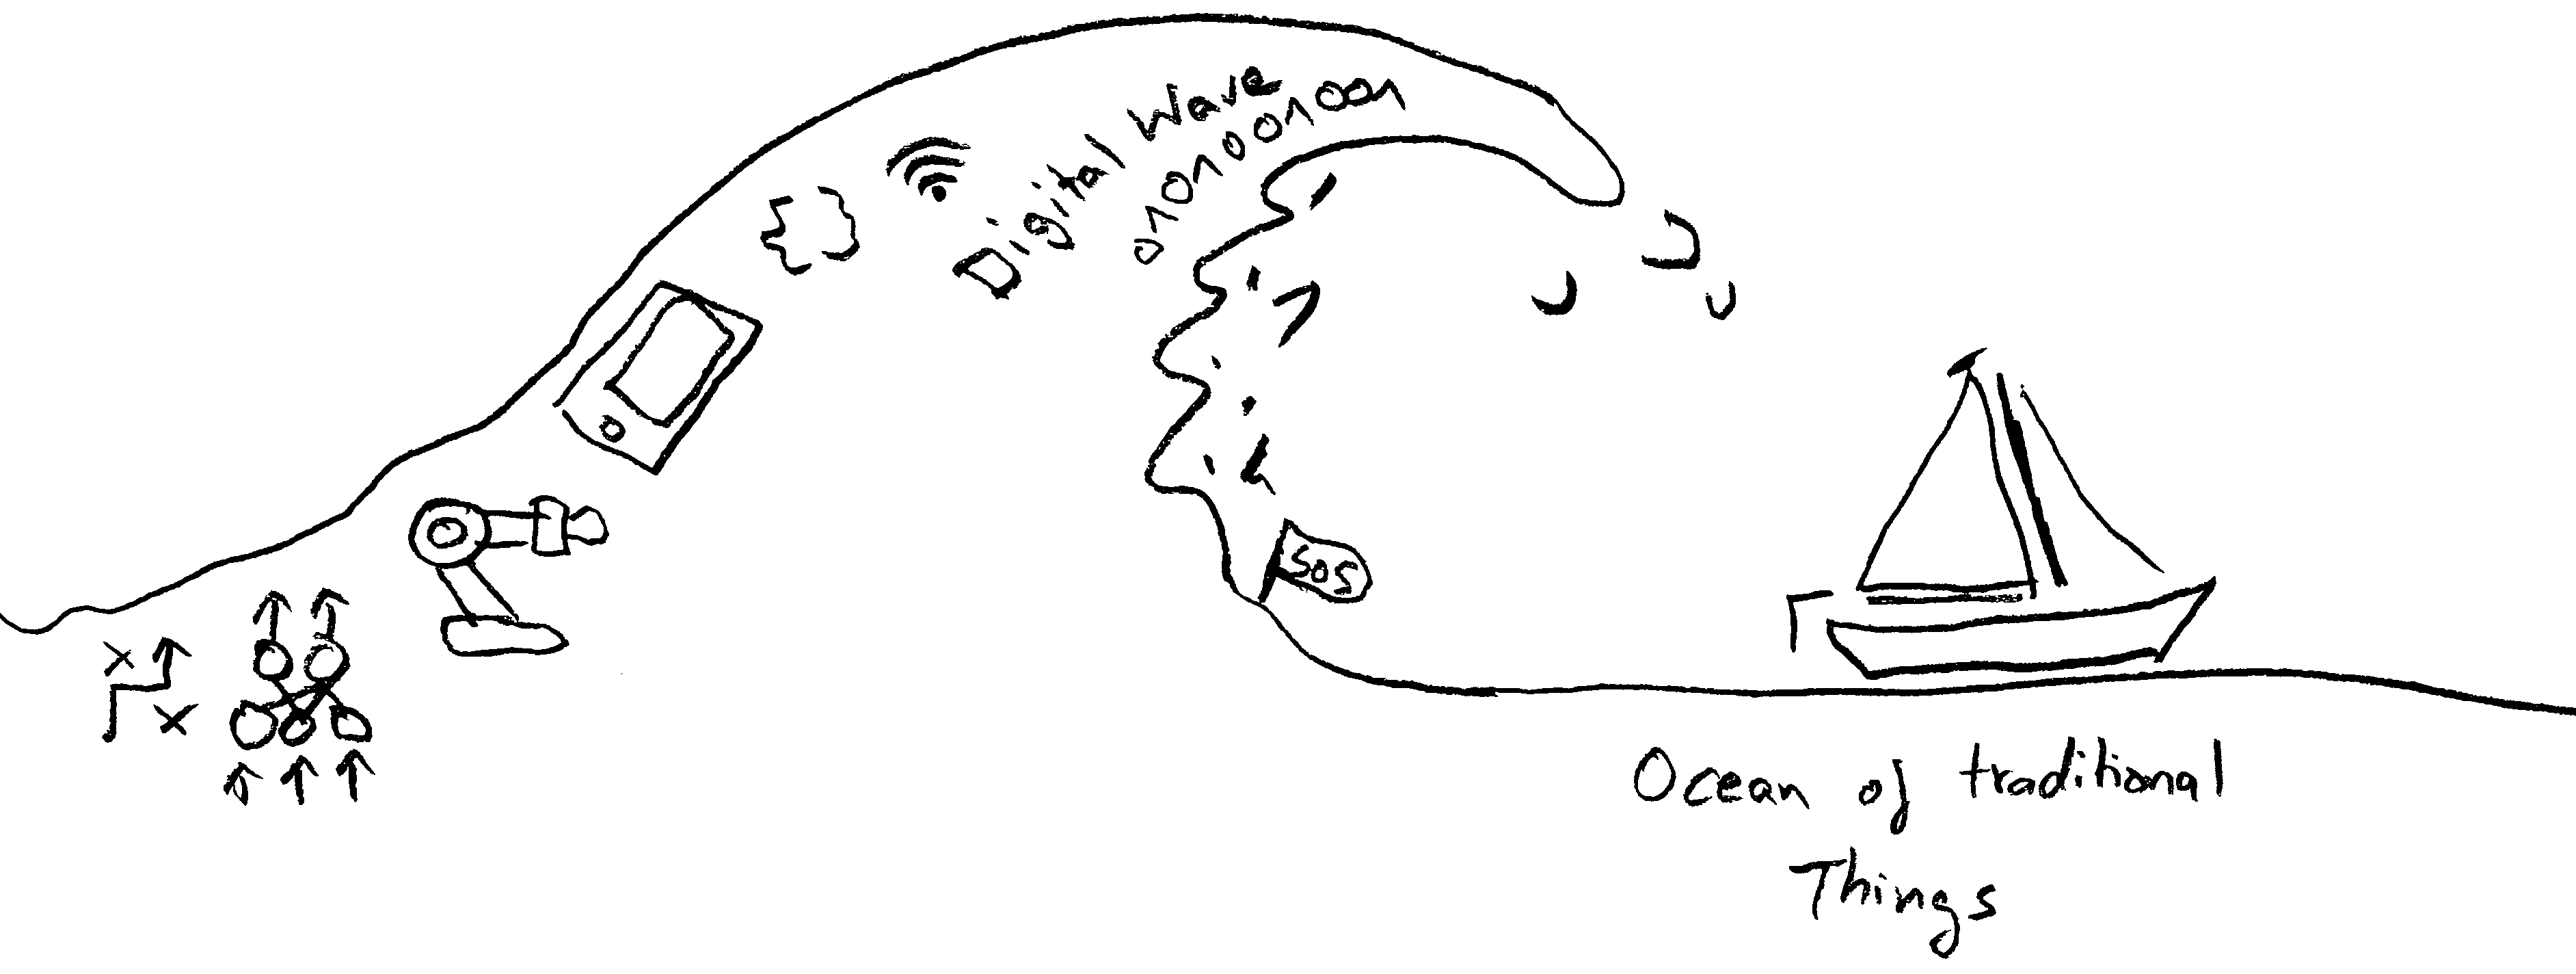
\includegraphics[width=8cm]{Digital_Wave_and_the_Ocean_of_Traditional_Things.png}
\caption{The Digital and the Ocean of Traditional Things, Florian Thiery [CC BY 4.0]}
\label{figdigitalwave}
\end{center}
\end{figure}

Thus, science and archaeology should seek collaboration with companies to positively influence the state and society through digital technologies. But does the digital wave overtake us? (Fig.~\ref{figdigitalwave}) We should surf the wave! On a first wave of digitalisation we have already recorded, saved, transmitted and processed machine-readable data via internet and cloud computing technologies. Furthermore, on the second wave of digitalisation we have to analyse, enhance and use these research data in active ways as machine-interpretable data using artificial intelligence and machine learning.

While surfing the waves, we actively experience the evolution of archaeology from analogue data to Knowledge Graph Computing. That is what I will call Archaeology 4.0 (Fig.~\ref{figa40pyramid}).

\begin{figure}[!htb]
\begin{center}
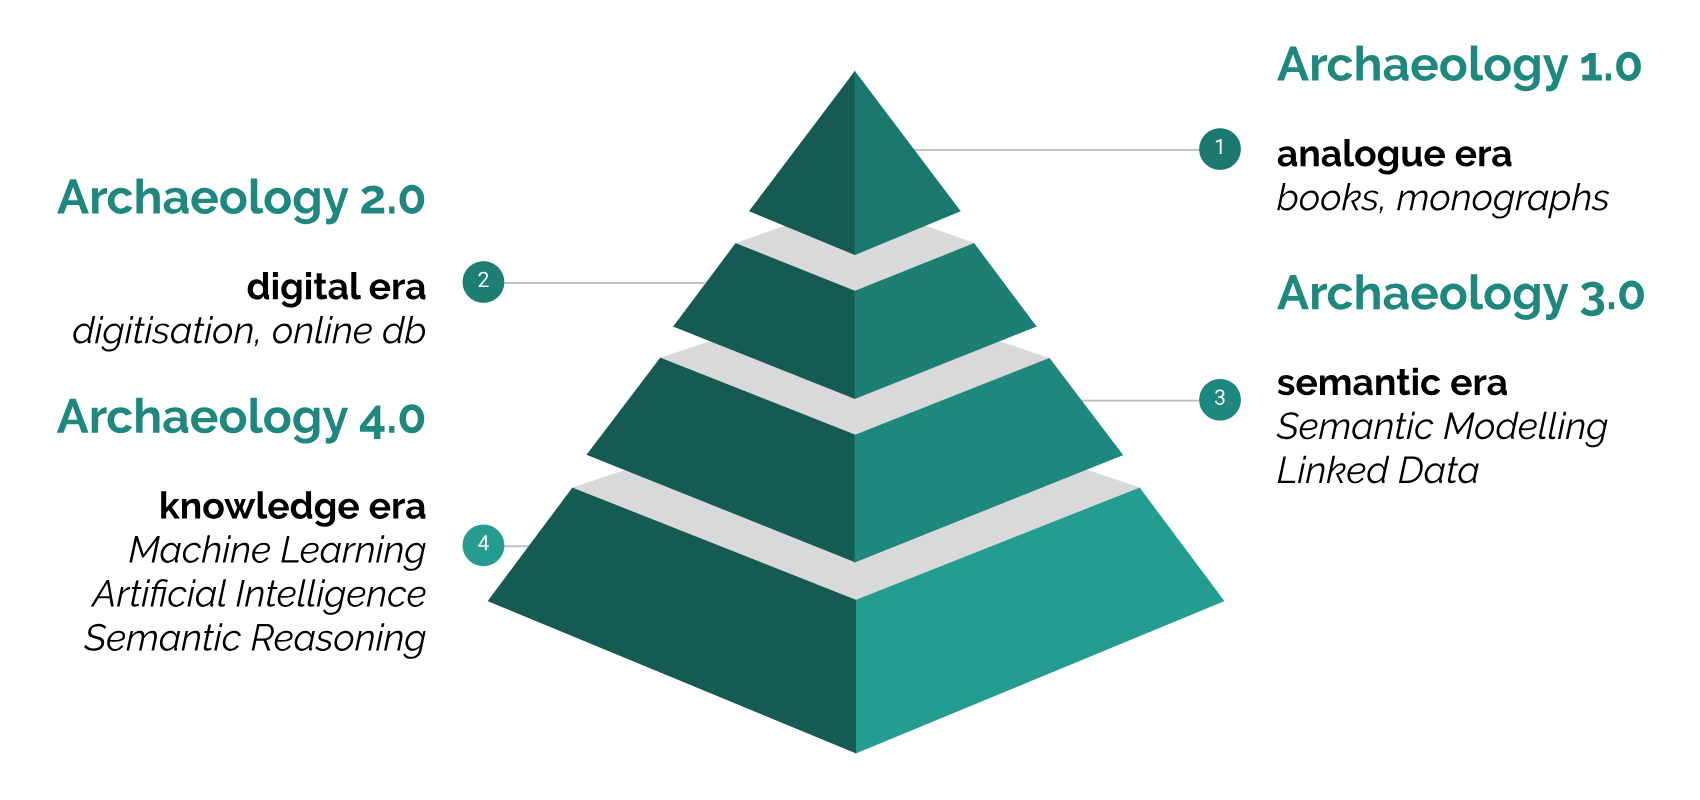
\includegraphics[width=8cm]{Archaeology_40.png}    
\caption{Archaelogy 4.0, Florian Thiery [CC BY 4.0]}  
\label{figa40pyramid}                               
\end{center}                                
\end{figure}

Archaeologal Sciences fulfilled a digital transformation from an 'analogous science' to modern digital science of humanities. Starting from an \textit{analogue era} (Archaeology 1.0), in which research data was kept in books and monographs, across the \textit{digital era} (Archaeology 2.0) in which digitisation progresses and data are published on the WWW, to a \textit{semantic era} (Archaeology 3.0), where semantic modelling and publication of Linked Data prevail, we end up in a \textit{knowledge era} (Archaeology 3.0), in which the analysis and the creation of new knowledge through a machine results.

\subsection{Archaeology 1.0}

\begin{figure}[!htb]
\begin{center}

\includegraphics[height=2cm]{a10.png}   
\caption{Archaelogy 1.0 Symbol, pixabay [Pixabay License]} 
\label{figa10symbol}                               
\end{center}                        
\end{figure}

I will call the era of non digital things ('analogue') the \textit{analogue era}. Research, and its underlying data, was published in printed books and monographs. Data access was only possible via active visiting libraries or complicated interlibrary loan. Research Data was not 'OPEN' at this time, because it was a privilege of an individual. 

\subsection{Archaeology 2.0}

\begin{figure}[!htb]
\begin{center}
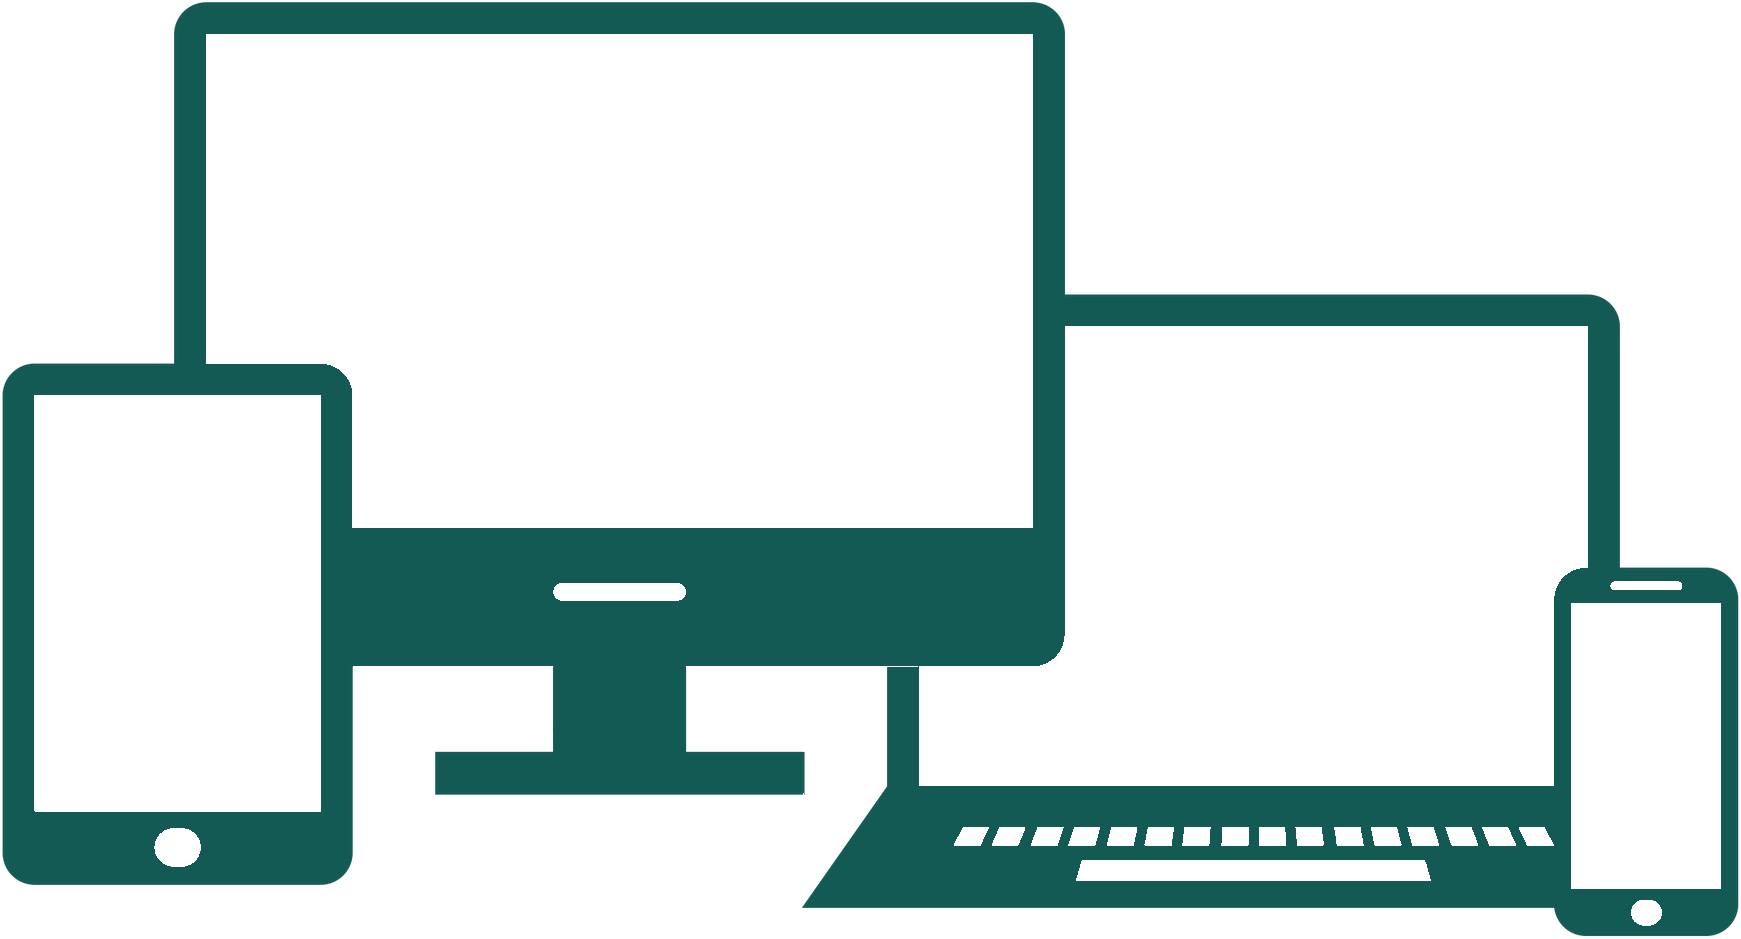
\includegraphics[height=2cm]{a20.png}
\caption{Archaelogy 2.0 Symbol, pixabay [Pixabay License]}
\label{figa20symbol}                                 
\end{center}                                
\end{figure}

I will call the time using and creating digital things the \textit{digital era}. With the invention of the Internet in $\approx$1969 by Vinton Gray Cerf ('father of the internet') and others and the invention of the World Wide Web in 1989 by computer scientist Sir Tim Berners-Lee and the so born Web 1.0, digital methods in archaeology come into play. (Archaeological) Research Data is from now on not exclusive any more, it is accessible for everyone via searchable online databases or PDF documents. The Web 2.0 including its so called 'Social Media' and the collaborative potential like Wikipedia and Google Docs enlarge the odds of shared archaeological research around the globe. The new possibilities of digitalisation methods of photographs and 3D documentation, using image analysis and 3D techniques, expand the range even more. Moreover, Open Data initiatives and common data format standards like the OGC web services, the Text Encoding Initiative (TEI) help to make research data interoperable, transparent and reproducible. This enables researcher using computer applications and quantitive methods to generate there own analyses via using digitised data.

\subsection{Archaeology 3.0}

\begin{figure}[!htb]
\begin{center}
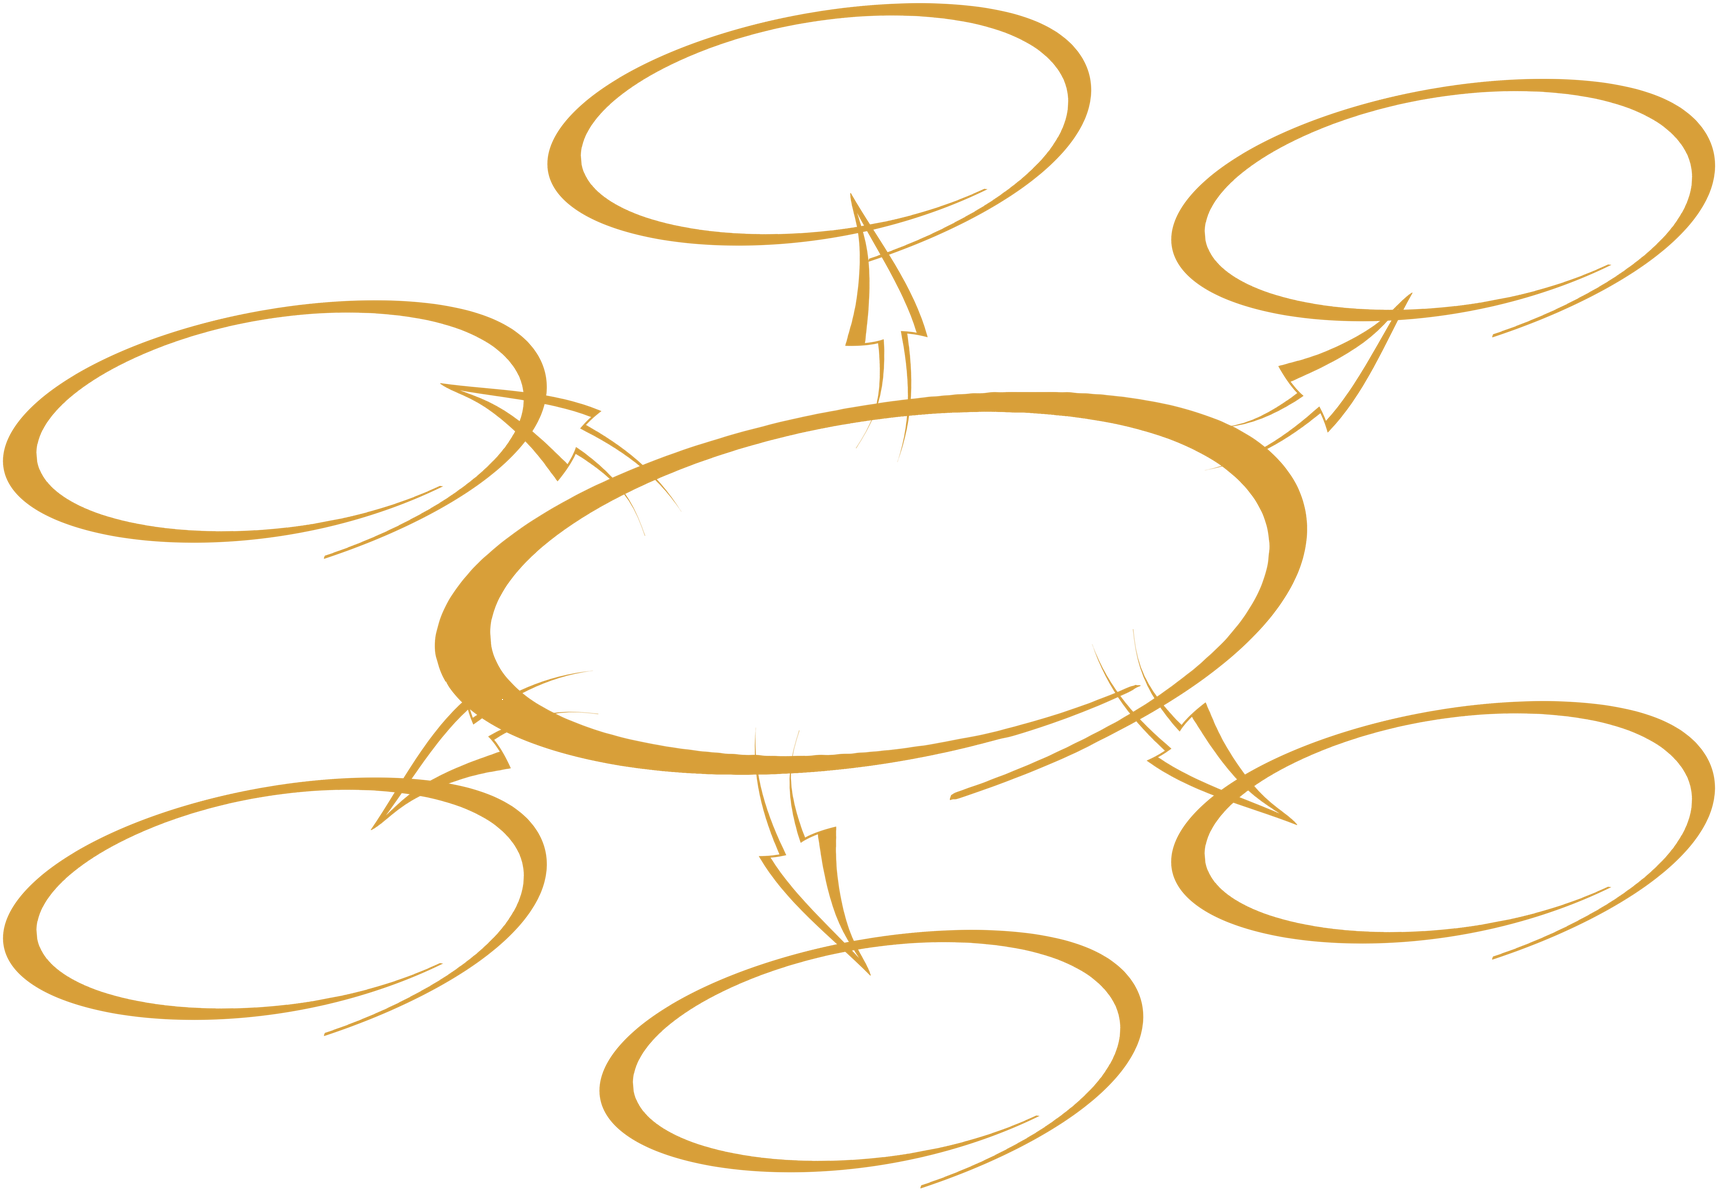
\includegraphics[height=2cm]{a30.png}
\caption{Archaelogy 3.0 Symbol, pixabay [Pixabay License]}
\label{figa30symbol}
\end{center}
\end{figure}

I will call the period of modelling data in graph and triple structures the \textit{semantic era}. In this era not only the structure matters - like in relational databases - the semantic meaning of things and their relationships are the backbone of research and scientific data. The idea of a Web 3.0, the so called Semantic Web comes into play. By the invention of a simple Resource Description Framework - RDF - everything stared. The RDF model is a data model based on a directed graph, were data are statements about resources. This statements are modelled as triples. A triple is modelled like a short sentence: Subject - Predicate - Object. Subject and Object are modelled as nodes, the predicate is the name of the directed edge between Subject and Object. Subjects and Predicates are usually URIs, Objects can be also a Literal, which are not unique. The base of the Semantic Web are ontologies. This big conceptual models including several axioms and rules to enable reasoning are usually modelled in the Web Ontology Language - OWL. The most common ontology in archaeology is the CIDOC CRM and its extensions.

\begin{figure}[!htb]
\begin{center}
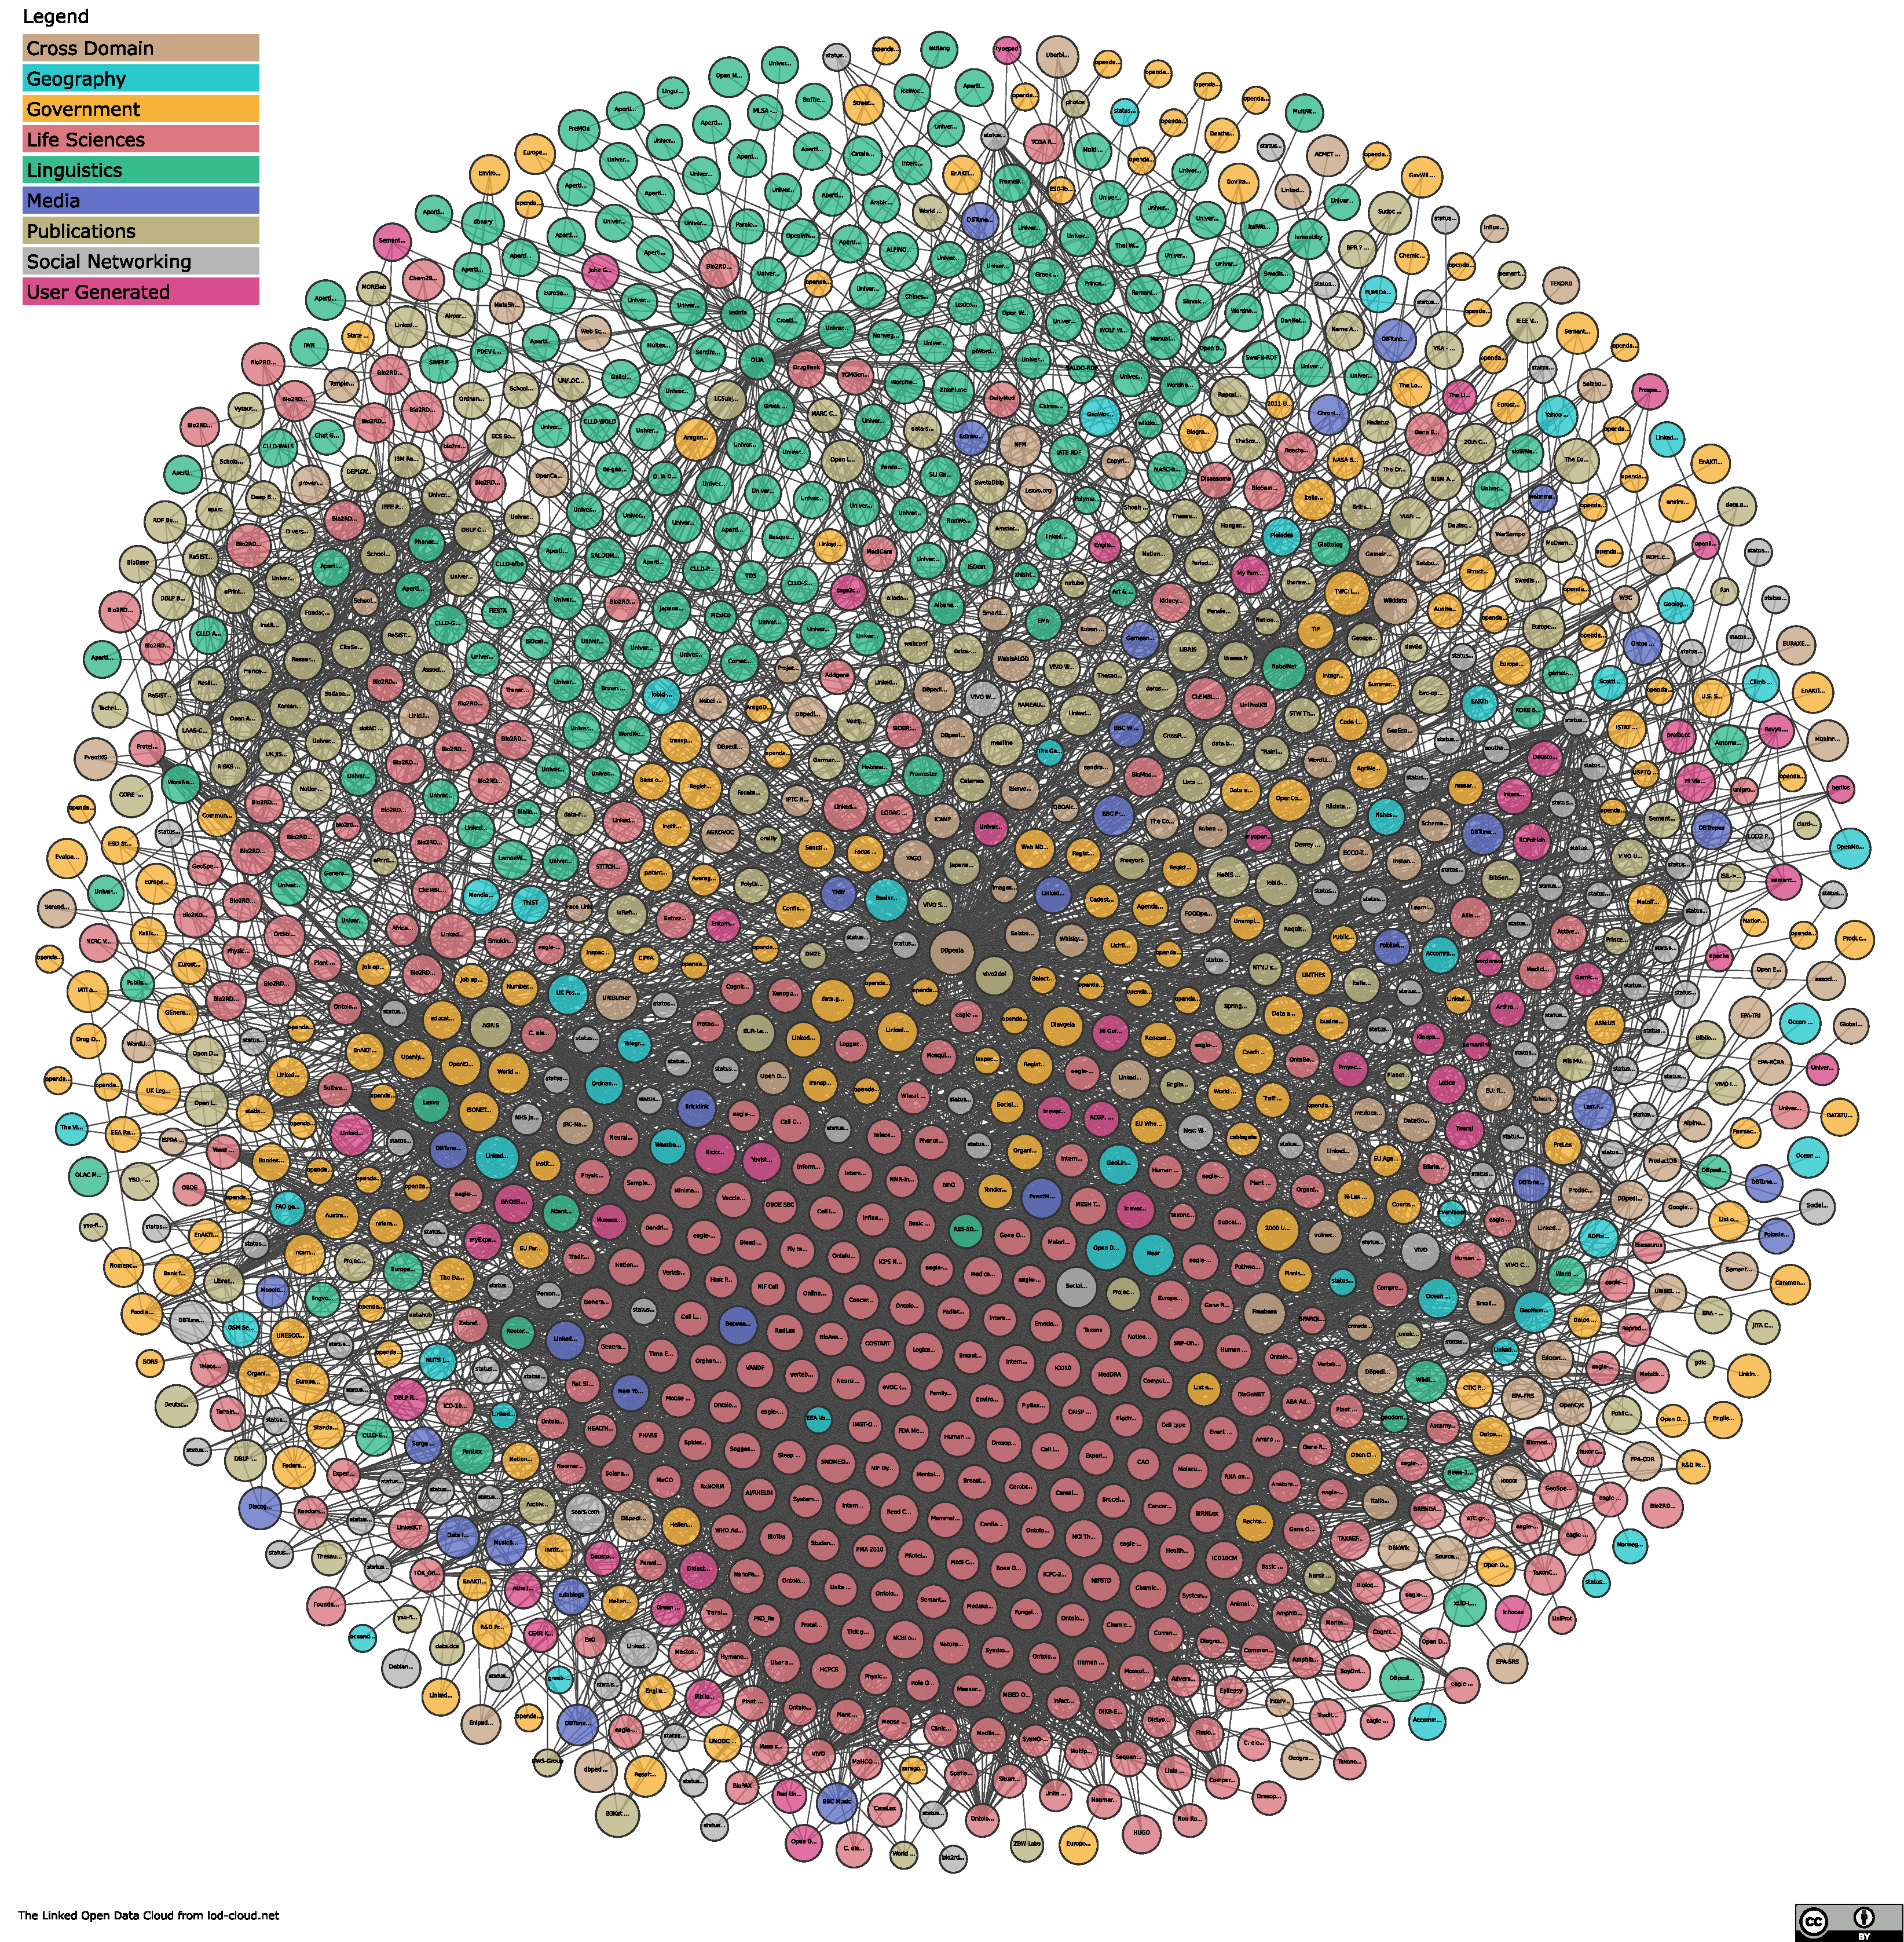
\includegraphics[width=8cm]{lod-cloud.pdf}
\caption{Linked Open Data Cloud 2019-03-29, lod-cloud.net [CC BY 4.0]}
\label{figlodc}
\end{center}
\end{figure}

Publishing data using the RDF data model ends up in using Linked Data. Tim Berners-Lee created four Linked Data rules \cite{bernerslee_linkeddata} for creating a Linked Data Cloud (Fig.~\ref{figlodc}): (1) use URIs as names for things, (2) use HTTP URIs so that people can look up those names, (3) when someone looks up a URI, provide useful information, using the standards like RDF and SPARQL, (4) include links to other URIs, so that they can discover more things.

\begin{figure}[!htb]
\begin{center}
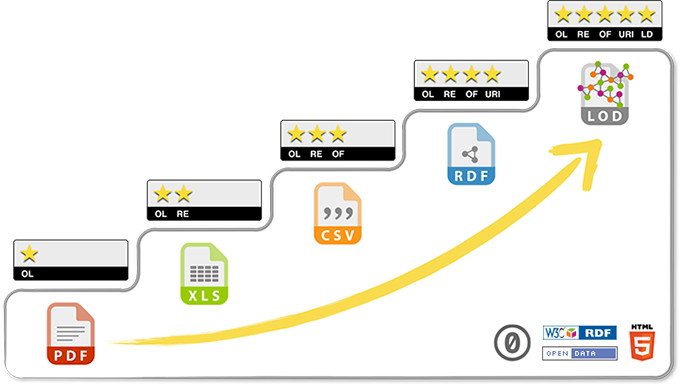
\includegraphics[width=8cm]{5-star-steps.png}
\caption{5 Star Open Data, 5stardata.info [CC0]}
\label{figfivestar}
\end{center}
\end{figure}

Mentioned in Archaeology 2.0, data is only usable if data will be shared and is open. Berners Lee also proposed the five star data model (Fig.~\ref{figfivestar}) for open data where Linked Data will be the best option, the so called Linked Open Data \cite{hausenblas_5star}.

To make Linked Data and Linked Open Data usable for computer scientists and researcher the term of LOUD - Linked Open Usable Data \cite{sanderson_loud} by Rob Sanderson was established into the Web 3.0 community. LOUD can also be devided into five design principles / stars, the ABCDE model: (1) the right \textit{Abstraction} for the audience, (2) few \textit{Barriers} to entry, (3) \textit{comprehensible} by introspection, (4) \textit{documentation} with working examples and (5) few \textit{Exceptions}, many consistent patterns.

The Web offers a lot of Linked Open Data in different domains (space, time, persons, keywords, ...) to use them for several purposes: LOD as Infrastructure, LOD as Research Data, LOD as Research Tool and LOD as Cloud. Resources can be found in several projects in the WWW like GeoNames, Pleiades, Pelagios, ChronOntology, Getty, Nomisma, ... Examples in archaeology are described in a famous PhD by Leif Isaksen "Archaeology and the Semantic Web" \cite{isaksen_archaeology} and in my own master thesis \cite{thiery_geinarfa}.

There are also some nice little projects build up in Mainz, Germany, for LOD as Infrastructure purposes (Labeling System, RGZM Meta-Index), for LOD as Research Data purposes (NAVIS 2.0, ARS3D), for LOD as Reseach Tool (Alligator, Academic Meta Tool) to establish a small piece of LOD as Cloud.

\begin{figure}[!htb]
\begin{center}
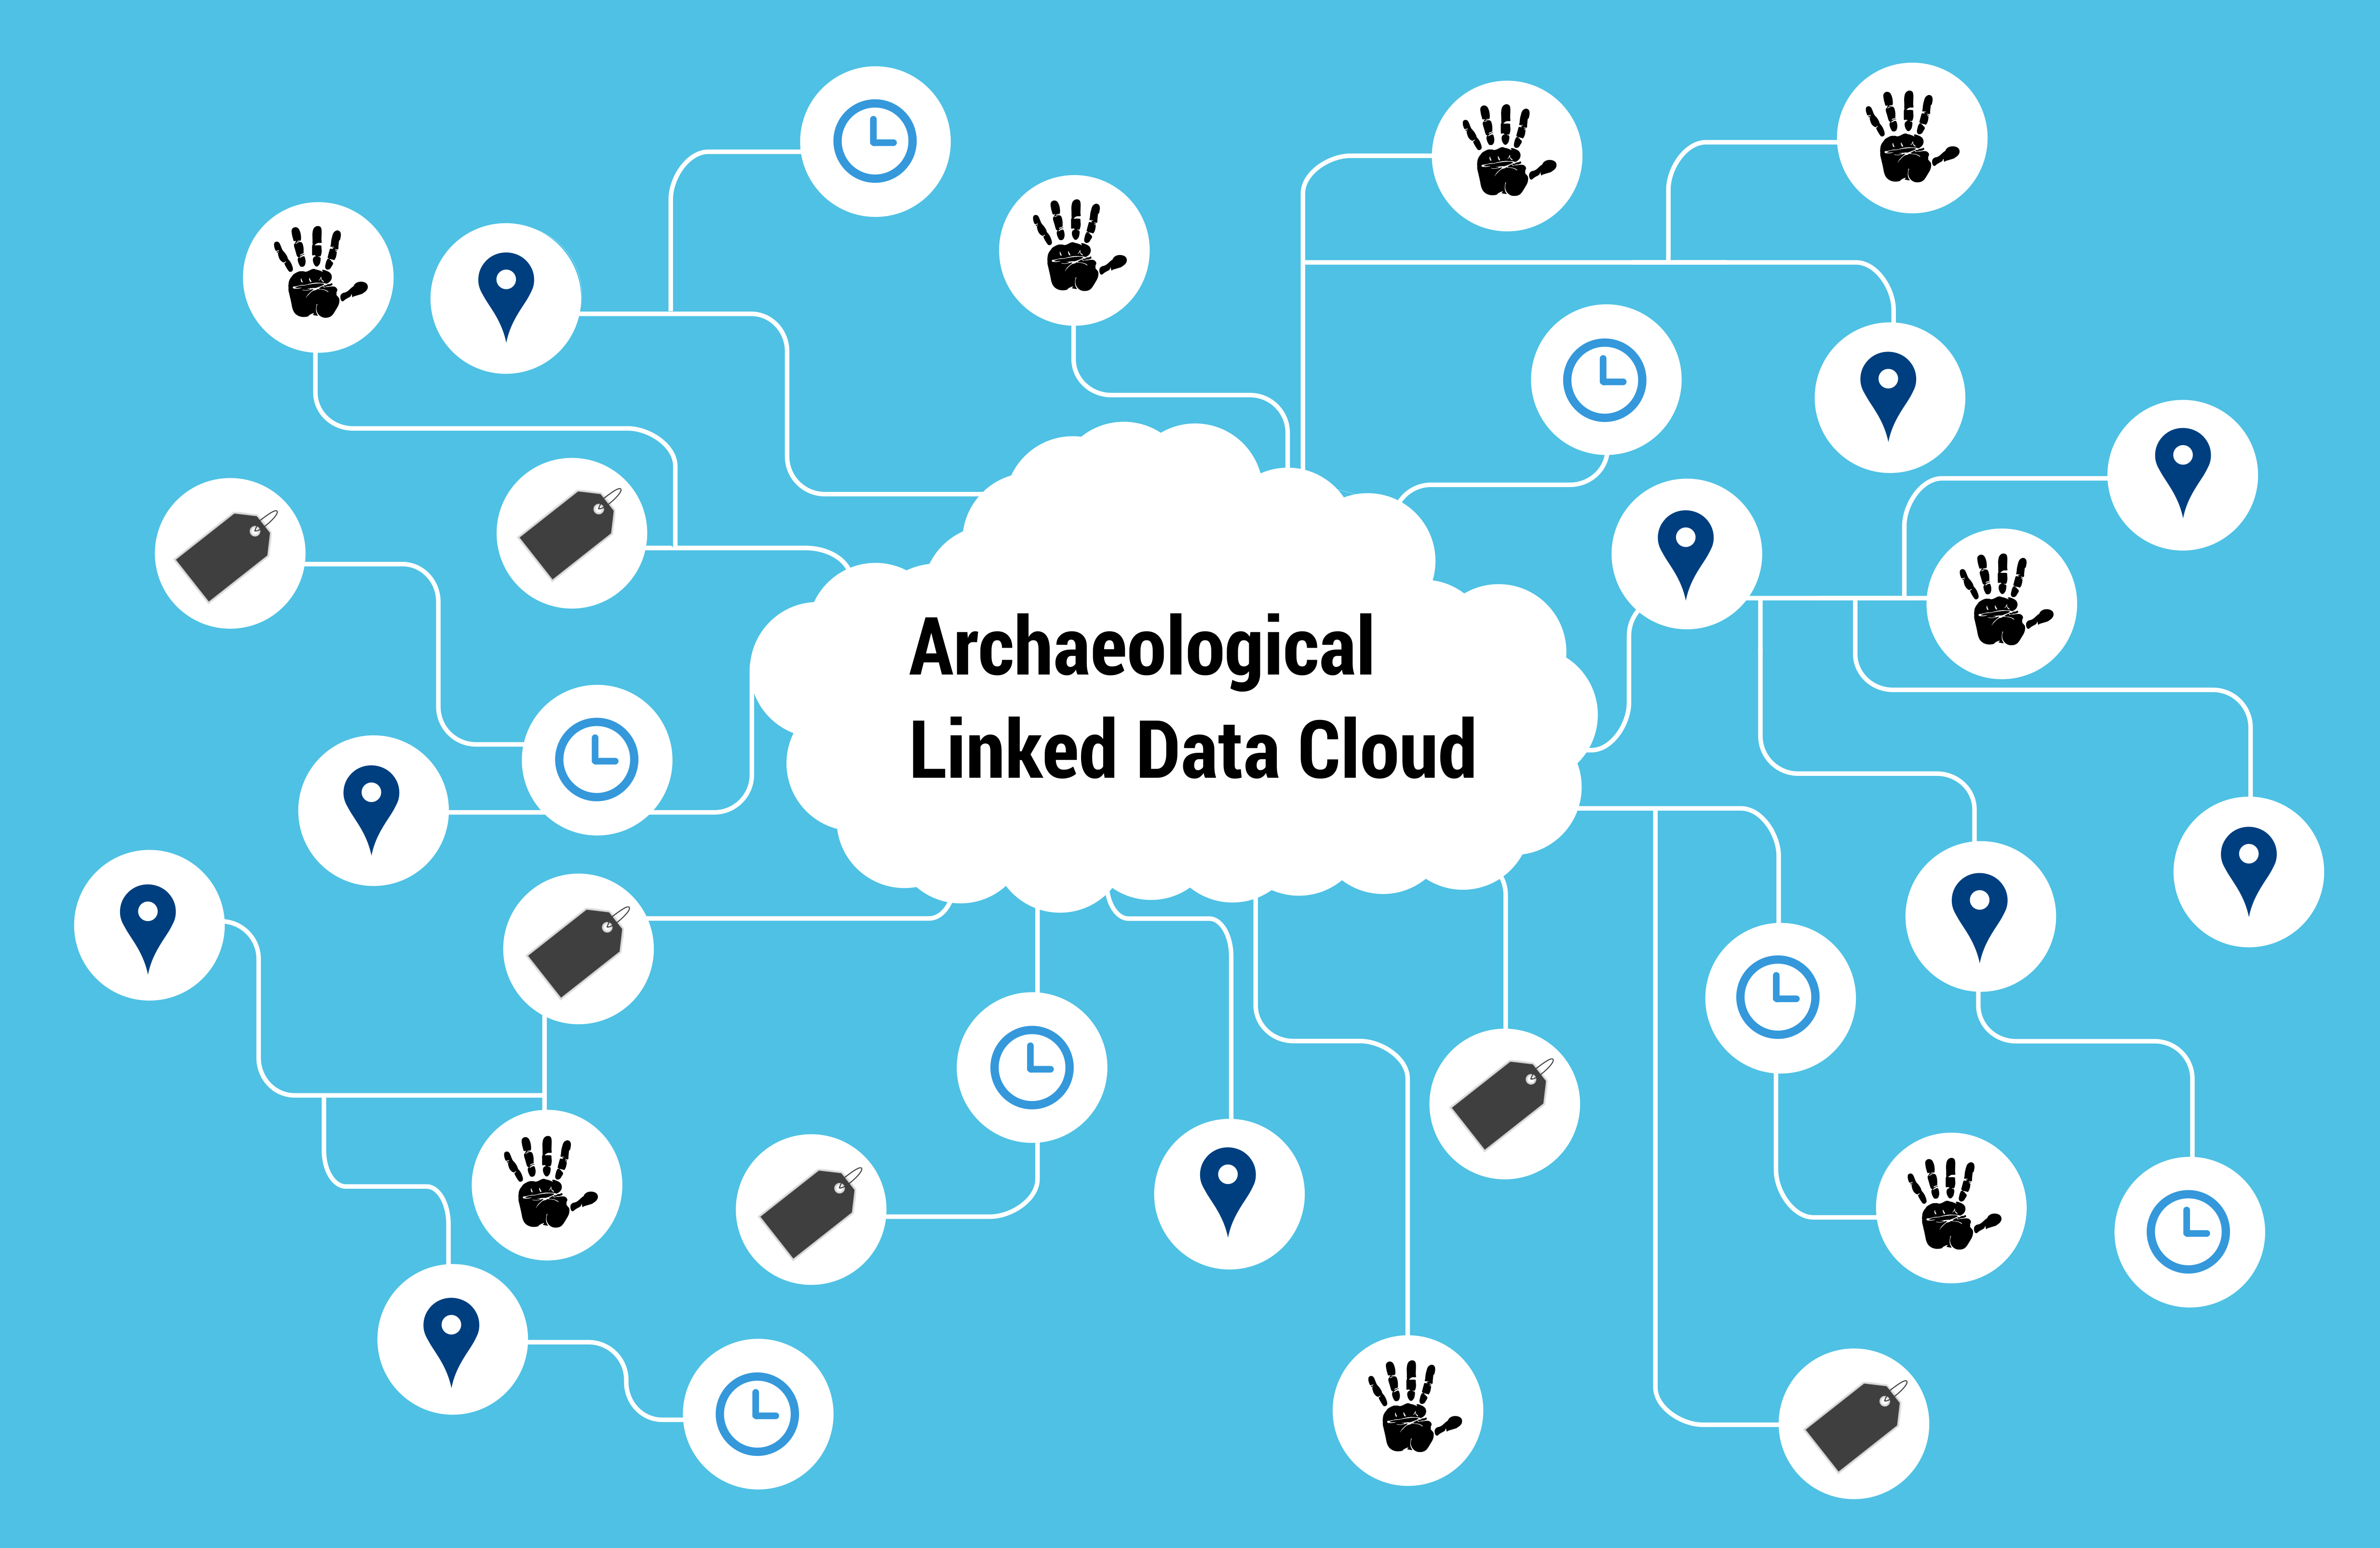
\includegraphics[width=8cm]{Archaeological_Linked_Data_Cloud_(ALDC).png}
\caption{Archaeological Linked Data Cloud, Florian Thiery [CC BY 4.0]}
\label{figaaldc}
\end{center}
\end{figure}

As the big aim of the archaeological Linked Open Data community, creating a Archaeological Linked Data Cloud comes into play (Fig.~\ref{figaaldc}). This cloud, including all archaeological object data, research data, meta data, para data with all of its hidden assumptions as well as interpretations in an objective, comprehensible, transparent and interoperable machine readable semantic way will open up new possibilities.

\subsection{Archaeology 4.0}

\begin{figure}[!htb]
\begin{center}
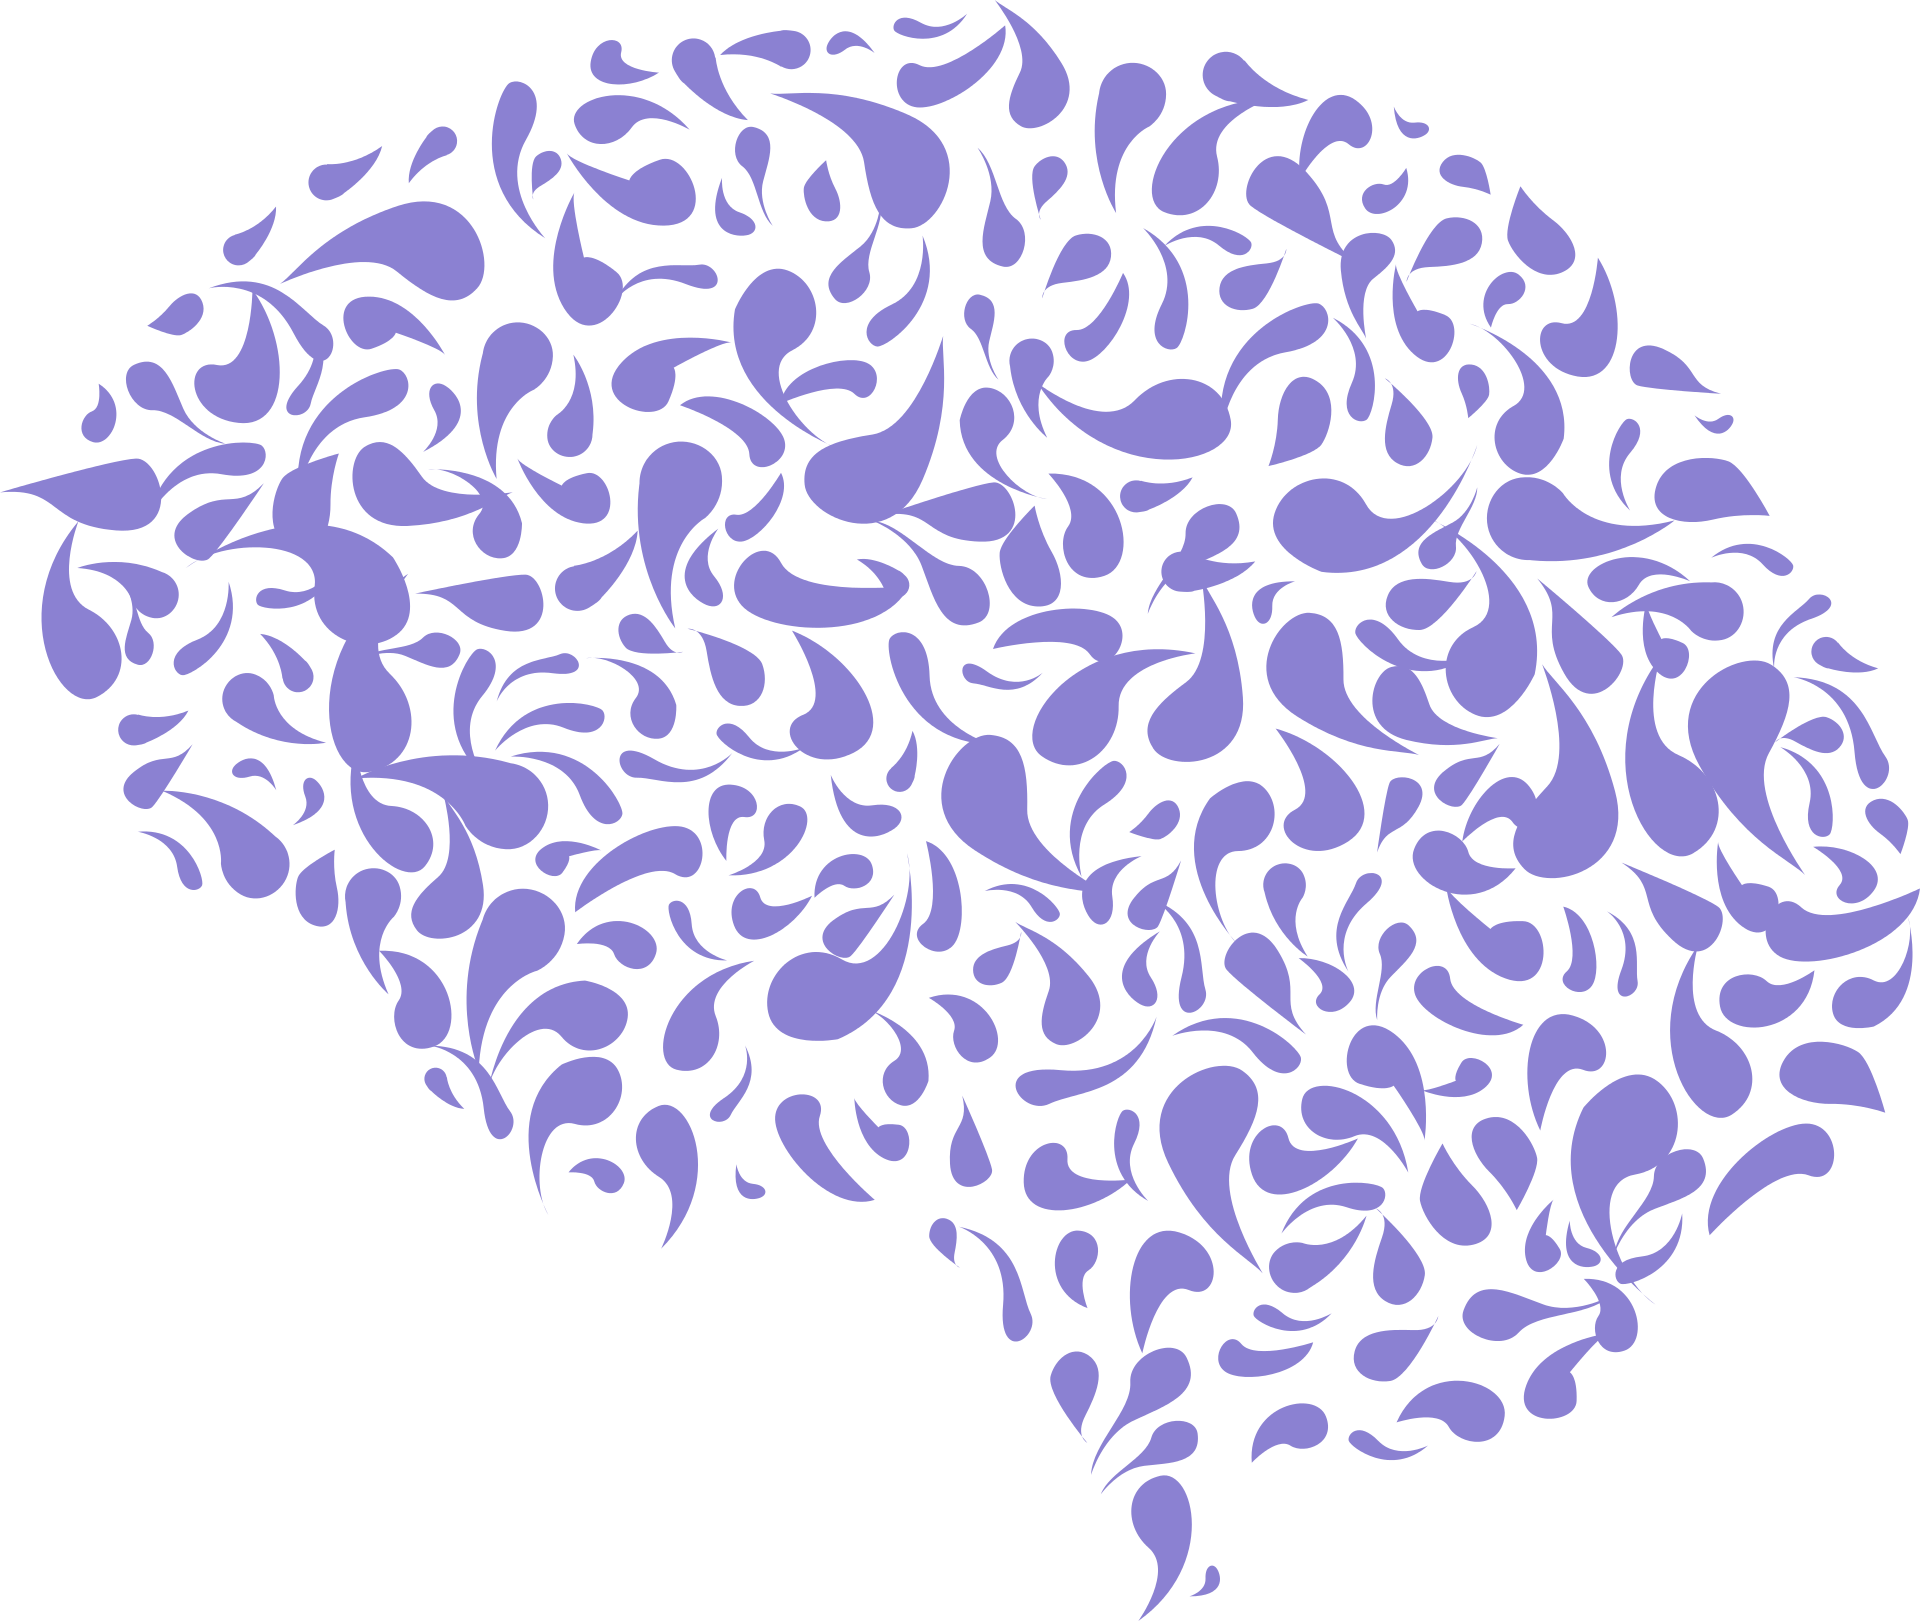
\includegraphics[height=2cm]{a40.png}    % The printed column  
\caption{Archaelogy 4.0 Symbol, pixabay [Pixabay License]}  % width is 8.4 cm.
\label{figa40symbol}                                 % Size the figures 
\end{center}                                 % accordingly.
\end{figure}

Lorem ipsum dolor sit amet, consetetur sadipscing elitr, sed diam nonumy eirmod tempor invidunt ut labore et dolore magna aliquyam erat, sed diam voluptua. At vero eos et accusam et justo duo dolores et ea rebum. Stet clita kasd gubergren, no sea takimata sanctus est Lorem ipsum dolor sit amet. Lorem ipsum dolor sit amet, consetetur sadipscing elitr, sed diam nonumy eirmod tempor invidunt ut labore et dolore magna aliquyam erat, sed diam voluptua. At vero eos et accusam et justo duo dolores et ea rebum. Stet clita kasd gubergren, no sea takimata sanctus est Lorem ipsum dolor sit amet. Lorem ipsum dolor sit amet, consetetur sadipscing elitr, sed diam nonumy eirmod tempor invidunt ut labore et dolore magna aliquyam erat, sed diam voluptua. At vero eos et accusam et justo duo dolores et ea rebum. Stet clita kasd gubergren, no sea takimata sanctus est Lorem ipsum dolor sit amet. 

Problem 

Techniken der Archäologie
4.0 benötigen oft große
Mengen an Trainingsdaten,
(“BigData”) die in der
Archäologie (noch) nicht
vorhanden sind.

Daten mittels Archäologie 3.0
semantisch u archäologisch
korrekt mit Metadaten
beschreiben UND verlinken,
so dass eine verlinkte
Archäologische Data Cloud
als breitere Basis für
Trainingsdaten entsteht.

\cite{mccreary_computing}

\cite{hey_computing}

\begin{figure}[!htb]
\begin{center}
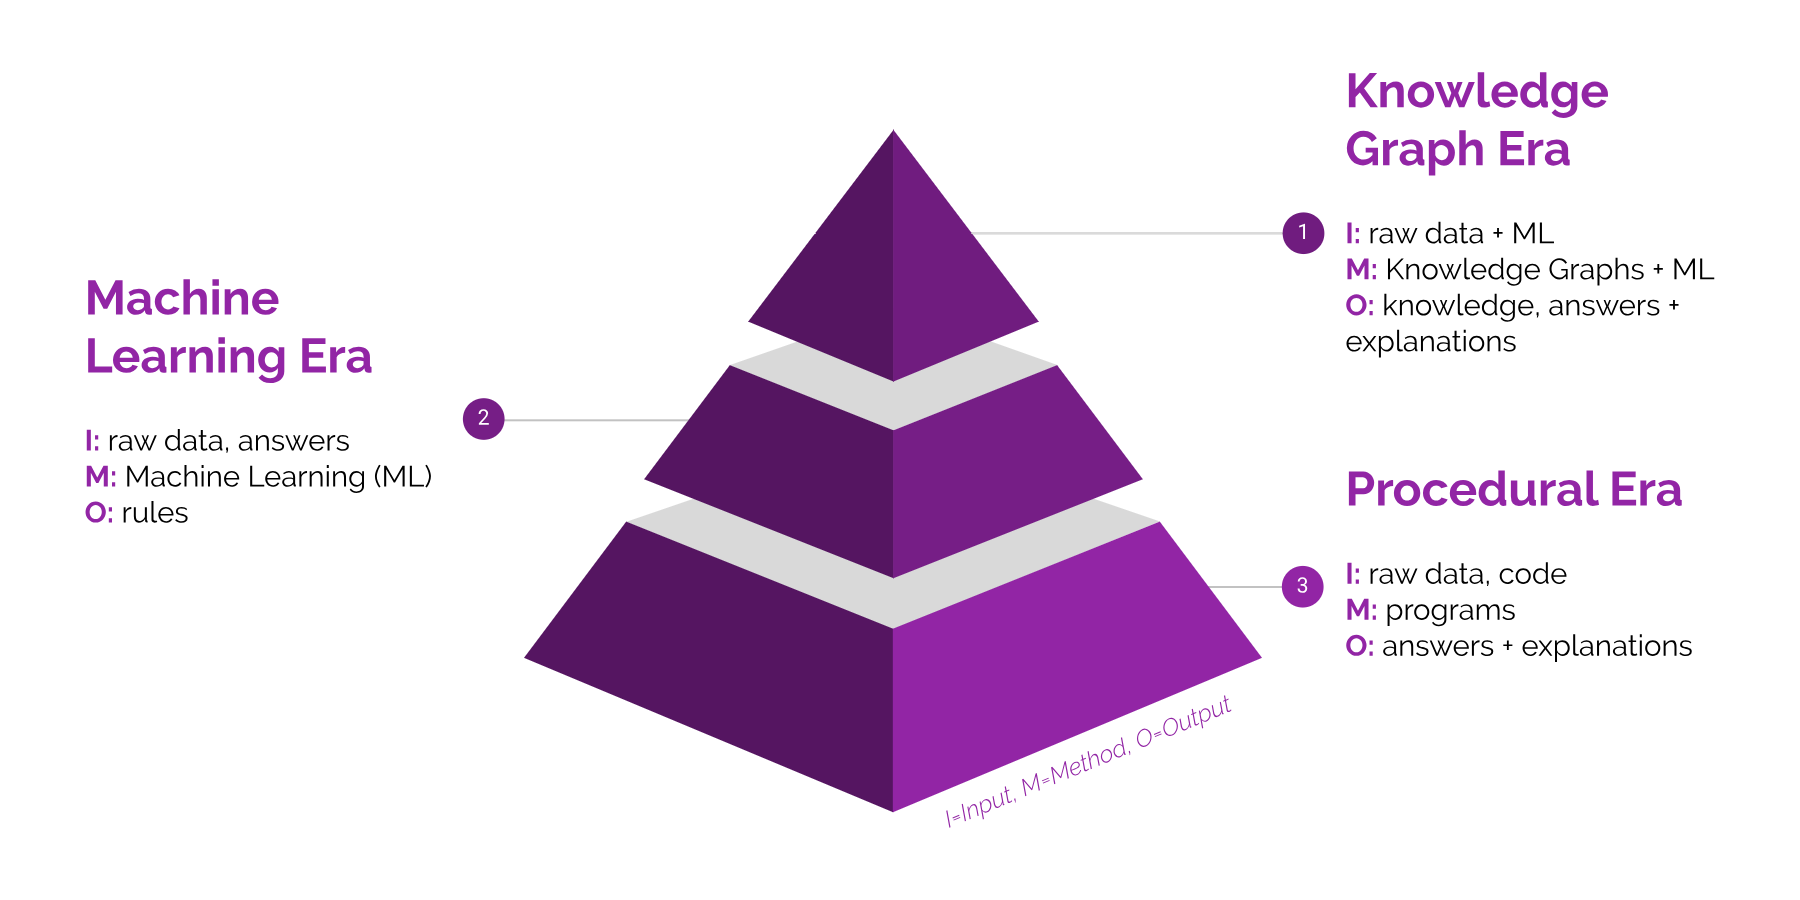
\includegraphics[width=8cm]{Era_of_Computing.png}    % The printed column  
\caption{Era of Computing, Florian Thiery [CC BY 4.0]}  % width is 8.4 cm.
\label{figeoc}                                 % Size the figures 
\end{center}                                 % accordingly.
\end{figure}

\begin{figure}[!htb]
\begin{center}
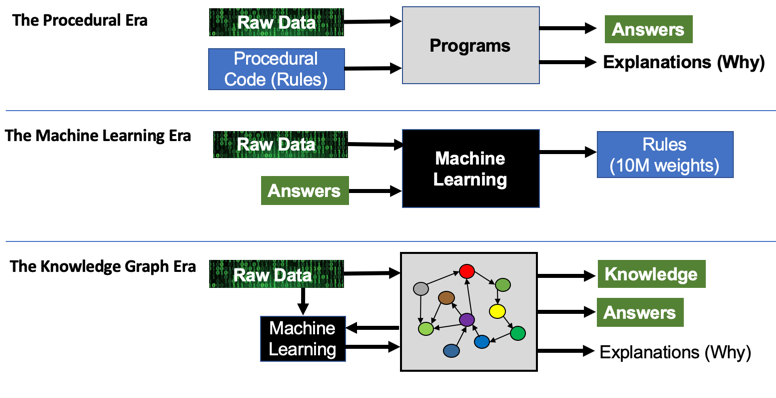
\includegraphics[width=8cm]{1_78b9DR1EApGRAst5FkPrwQ.png}    % The printed column  
\caption{Era of Computing, Dan McCreary \cite{mccreary_computing}}  % width is 8.4 cm.
\label{figeoco}                                 % Size the figures 
\end{center}                                 % accordingly.
\end{figure}

\begin{ack}                               
I would like to thank the Mainz Centre for Digitality in the Humanities and Cultural Studies (mainzed) and R\"omisch-Germanisches Zentralmuseum. In particular Prod. Dr. Kai-Christian-Bruhn (ORCID: 0000-0001-8322-1260) and Dr. Allard Mees FSA (ORCID: 0000-0002-7634-5342).
\end{ack}

\bibliographystyle{plain}        % Include this if you use bibtex 
\bibliography{autosam}           % and a bib file to produce the 
                                 % bibliography (preferred). The
                                 % correct style is generated by
                                 % Elsevier at the time of printing.

\end{document}